% \documentclass{beamer}
\documentclass[xcolor=dvipsnames]{beamer}
%% \usecolortheme[named=Blue]{structure}
\setbeamersize{text margin left=30mm, text margin right=30mm}
\useoutertheme{infolines}
\usetheme[height=7mm]{Rochester}
\setbeamertemplate{items}[ball]
\setbeamertemplate{blocks}[rounded][shadow=true]
\setbeamertemplate{navigation symbols}{}

\usepackage[utf8x]{inputenc}
\usepackage{default}
\usepackage[english]{babel}
\usepackage{geometry}
%% \usepackage{fullpage}
\usepackage{amsmath, amsthm, amssymb}
\usepackage{listings}
\usepackage{pxfonts}
%% \usepackage{color}
%% \usepackage{graphicx}
%% \usepackage{natbib}
%% \usepackage{array}
%% \usepackage{booktabs}
%% \usepackage{tabu}
%% \usepackage[utf8]{inputenc}
%% \usepackage{fancyhdr}
%% \usepackage{float}
%% \usepackage{subfigure}
%% \usepackage{titlesec}


\def\CCT{{C\nolinebreak[4]\hspace{-.05em}\raisebox{.4ex}{\tiny\bf ++}}}
\def\CC{{C\nolinebreak[4]\hspace{-.05em}\raisebox{.4ex}{\small\bf ++}}}


\definecolor{lstgray}{gray}{0.97}
\lstset{ %
  escapechar=@,
  language=C++,
  basicstyle=\footnotesize\ttfamily,
  %% basicstyle=\ttfamily,
  %% keywordstyle=\color{blue}\ttfamily,
  keywordstyle=\bfseries,
  stringstyle=\color{red}\ttfamily,
  commentstyle=\color{OliveGreen}\ttfamily,
  morecomment=[l][\color{red}]{\#},
  backgroundcolor=\color{lstgray},
  %% keywordstyle=\color{red},
  frame=f,
  frameround=ffff,
  tabsize=2,
  breaklines=true,
  breakatwhitespace=false,
  showspaces=false,
  showstringspaces=false,
  xleftmargin=5pt,
  xrightmargin=5pt,
  morekeywords={in,out,ref,auto,inout,import,ushort,scope,exit,mixin,decltype,varid,sizeof}
}

\def\redcolor{\color{red}}
\def\bluecolor{\color{blue}}
\def\blackcolor{\color{black}}
\def\graycolor{\color{gray}}
\def\greencolor{\color{OliveGreen}}


\def\sectionname{\translate{Section}}
\def\insertsectionnumber{\arabic{section}}
\setbeamertemplate{section page}
{
  \begin{centering}
    \begin{beamercolorbox}[sep=4pt,center]{part title}
      \usebeamerfont{section title}\insertsection\par
    \end{beamercolorbox}
  \end{centering}
}
\def\sectionpage{\usebeamertemplate*{section page}}


\AtBeginSection{\frame{\sectionpage}}


\title{Reflecting on names}
\subtitle{Facilitating expression tree transforms}
%% \author{\texorpdfstring{Author\newline\url{email@email.com}}{Dominic Jones}}
\author{Dominic Jones}
%% \author{Author\\{\tiny email@email.com}}
\institute{\texttt{dominic.jones@gmx.co.uk}}
\date{London, October 2017}


\begin{document}
\begin{frame}[plain]
  \titlepage
\end{frame}


\begin{frame}[fragile]{Same type, different name}
Write a \texttt{transform} function to yield:\vspace{10mm}
\begin{lstlisting}
  transform(@\aftergroup\bluecolor@a + a@\aftergroup\blackcolor@) -> @\aftergroup\redcolor@2 * a@\aftergroup\blackcolor@


  transform(@\aftergroup\bluecolor@a + b@\aftergroup\blackcolor@) -> @\aftergroup\bluecolor@a + b@\aftergroup\blackcolor@
\end{lstlisting}
\vspace{10mm}where {\color{blue}\texttt{a}} and {\color{blue}\texttt{b}} are of the \emph{same type}
\end{frame}


\begin{frame}[fragile]{Reflection}
  \begin{lstlisting}

@\aftergroup\graycolor@ 123456789 123456789 123456789
          10        20        30
1
2  // main.cpp
3
4@\aftergroup\blackcolor@  decltype(x)*   y   =   &x;@\aftergroup\graycolor@
5

@\aftergroup\greencolor@     reflect             reflect
     type                address@\aftergroup\graycolor@
  \end{lstlisting}
 \vspace{10mm}
Reflect location?
\end{frame}


\begin{frame}[fragile]{\texttt{varid}}
\begin{lstlisting}
template<typename Fn, typename L, typename R,
         @\aftergroup\bluecolor@std::size_t IL@\aftergroup\blackcolor@, @\aftergroup\bluecolor@std::size_t IR@\aftergroup\blackcolor@>
struct Binary
{
  Binary(L const &l, R const &r);
  ...
};


// declaration of `l' and `r' must be visible
template<typename L, typename R>
auto operator+(L const &l, R const &r)
-> Binary<Add, L, R, @\aftergroup\bluecolor@varid(l)@\aftergroup\blackcolor@, @\aftergroup\bluecolor@varid(r)@\aftergroup\blackcolor@>
{
  return {l, r};
}
\end{lstlisting}
\end{frame}


\begin{frame}[fragile]{Location stamped type}
\begin{lstlisting}
  decltype(@\aftergroup\bluecolor@a + a@\aftergroup\blackcolor@) -> Binary<Add, T, T, @\aftergroup\redcolor@5724, 5724@\aftergroup\blackcolor@>


  decltype(@\aftergroup\bluecolor@a + b@\aftergroup\blackcolor@) -> Binary<Add, T, T, @\aftergroup\bluecolor@5724, 1396@\aftergroup\blackcolor@>
\end{lstlisting}
\end{frame}


\begin{frame}[fragile]{Like \texttt{sizeof}}
  \begin{enumerate}
  \item keyword \vspace{5mm}
  \item evaluated at compile-time \vspace{5mm}
  \item returns an unsigned int \vspace{5mm}
  \end{enumerate}
\end{frame}


\begin{frame}[fragile]{Like ``\texttt{\&}'', address operator}
  \begin{enumerate}
  \item expects an l-value \vspace{5mm}
  \item returns ``something like'' an address: \vspace{5mm}
    \begin{itemize}
    \item hash of the {\color{blue}file name, row and column} of the referenced variable \vspace{5mm}
    \item traces to the referenced temporary or named variable \vspace{5mm}
    \end{itemize}
  \end{enumerate}
\end{frame}


\begin{frame}[fragile]{Valid uses}
\begin{lstlisting}
auto c0 = 3;
auto c1 = 4;


// compare visibly declared variables
static_assert(varid(c1) @\aftergroup\redcolor@!=@\aftergroup\blackcolor@ varid(c0));


// compare with const-referenced variable
auto const &cr = c0;
static_assert(varid(cr) @\aftergroup\bluecolor@==@\aftergroup\blackcolor@ varid(c0));


// compare with copied variable
auto const cc = c0;
static_assert(varid(cc) @\aftergroup\redcolor@!=@\aftergroup\blackcolor@ varid(c0));
\end{lstlisting}
\end{frame}


\begin{frame}[fragile]{Invalid uses}
\begin{lstlisting}
auto c0 = 3;
auto c1 = 4;


// error: expressions not supported
auto constexpr i0 = varid(@\aftergroup\redcolor@c0 * c1@\aftergroup\blackcolor@);


// error: literals not supported
auto constexpr i1 = varid(@\aftergroup\redcolor@3@\aftergroup\blackcolor@);


// error: types not supported
auto constexpr i2 = varid(@\aftergroup\redcolor@double@\aftergroup\blackcolor@);


// error: must be const-qualified
auto &cr = c0;
auto constexpr i3 = varid(@\aftergroup\redcolor@cr@\aftergroup\blackcolor@);
\end{lstlisting}
\end{frame}


\begin{frame}[fragile]{Workaround}
\begin{lstlisting}

template<std::size_t ID, typename T>
struct Unique { T value; };

// using non-standard macro...
#define UQ(v) Unique<__COUNTER__, decltype(v)>{v}


auto c0 = @\aftergroup\redcolor@UQ@\aftergroup\blackcolor@(3);
auto c1 = @\aftergroup\redcolor@UQ@\aftergroup\blackcolor@(4);

// compare visibly declared variables
static_assert(varid(c1) != varid(c0));

...
\end{lstlisting}
\end{frame}


\begin{frame}[fragile]{Actual use}
  \begin{itemize}
  \item Compile-time \emph{Automatic Differentiation} \vspace{5mm}
  \item Order of magnitude better performance \vspace{5mm}
  \item Clumsy to write with {\color{red}{\texttt{UQ}}} decorators \vspace{5mm}
  \end{itemize}
\end{frame}


\begin{frame}[fragile]{Duplicate branches?}
  \begin{columns}[T] % align columns
    \begin{column}{.49\textwidth}
        \begin{lstlisting}
auto eval(A const &a,
          B const &b)
{
  // statically identical?
  auto @\aftergroup\redcolor@c0@\aftergroup\blackcolor@ = 3;
  auto @\aftergroup\redcolor@c1@\aftergroup\blackcolor@ = 4;

  // `t0' evaluated twice?
  auto @\aftergroup\bluecolor@t0@\aftergroup\blackcolor@ = a * b;
  auto t1 = @\aftergroup\redcolor@c0@\aftergroup\blackcolor@ + @\aftergroup\bluecolor@t0@\aftergroup\blackcolor@;
  auto t2 = @\aftergroup\redcolor@c1@\aftergroup\blackcolor@ + @\aftergroup\bluecolor@t0@\aftergroup\blackcolor@;

  return t1 / t2;
}
  \end{lstlisting}
    \end{column}%
    \hfill%
    \begin{column}{0.49\textwidth}
\begin{figure}[H]
 \centering
 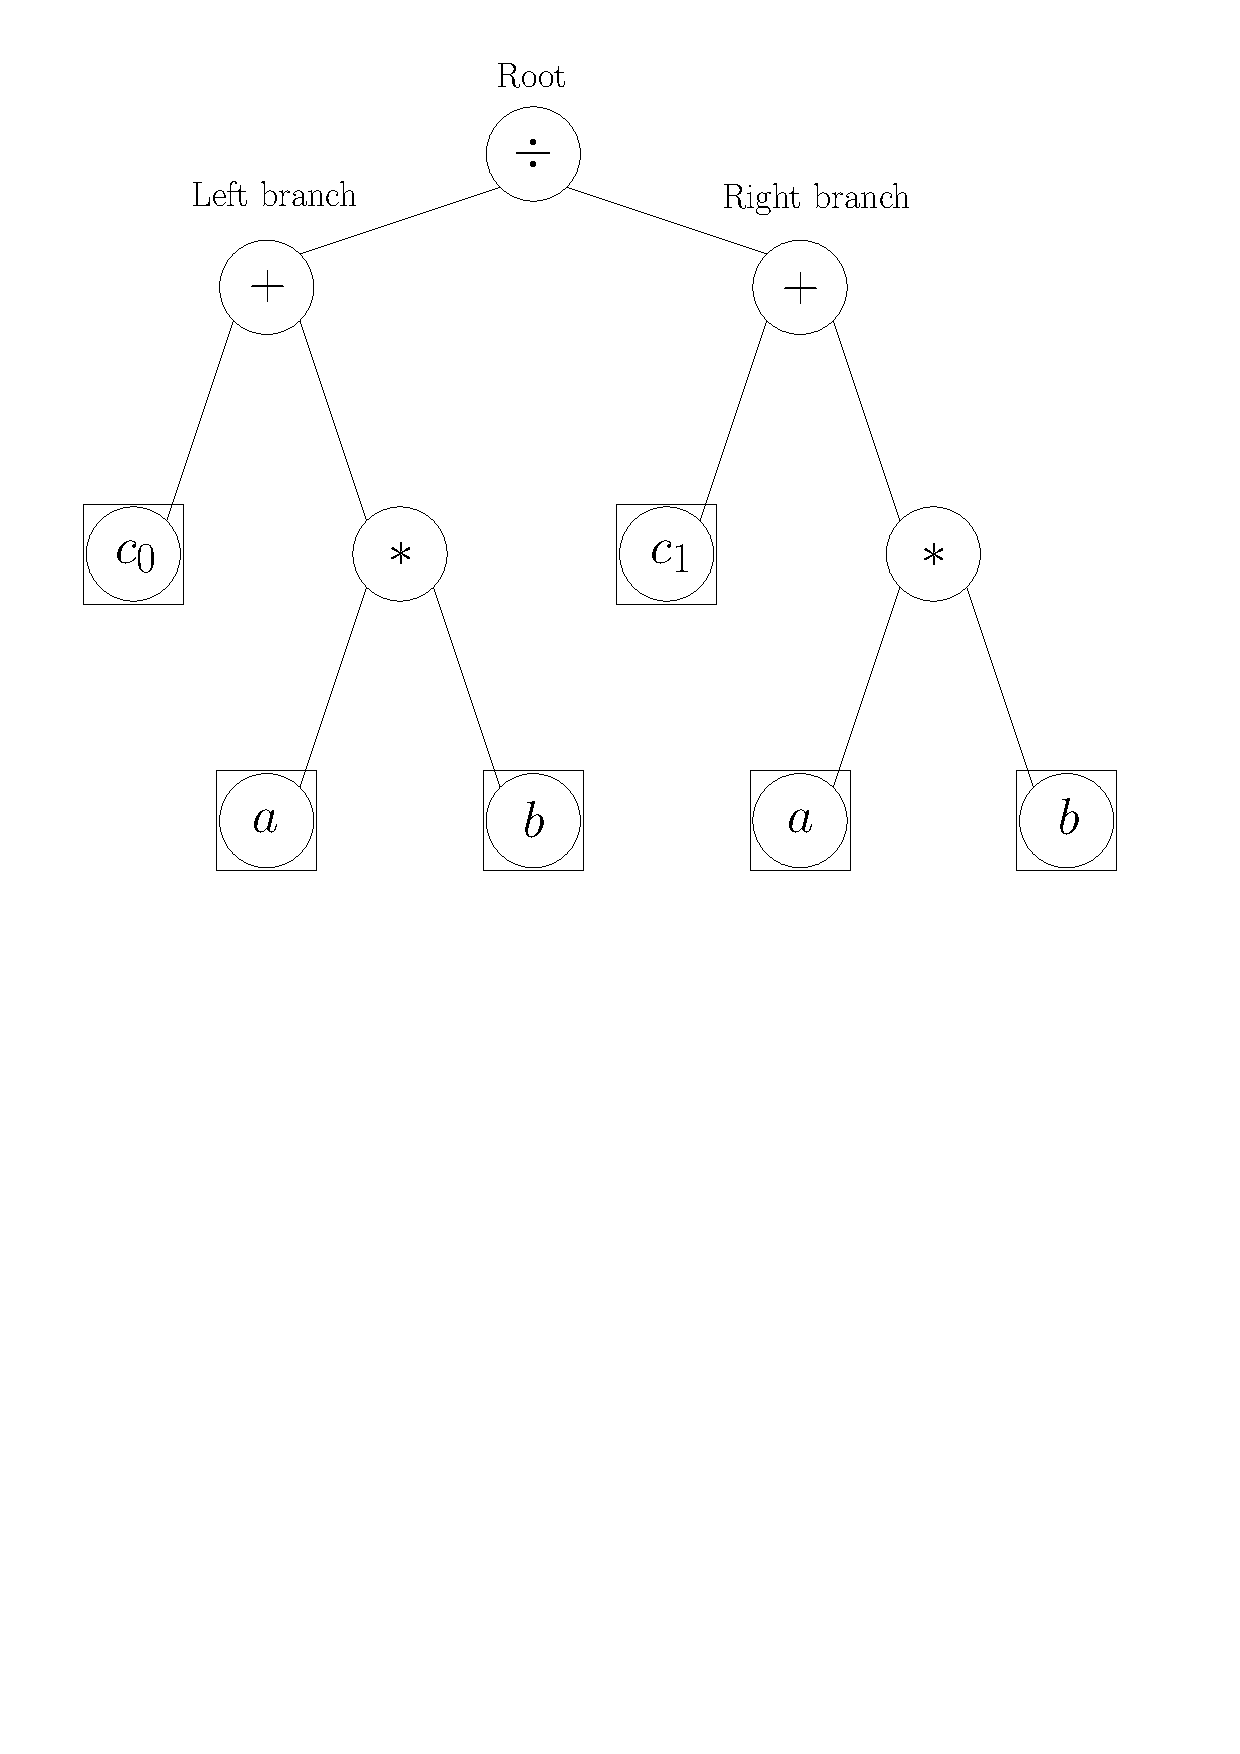
\includegraphics[width=0.99\textwidth]{fig_exprtree}
\end{figure}
    \end{column}%
  \end{columns}
\end{frame}


\begin{frame}[fragile]{Plan}
  \begin{enumerate}
  \item Implement \texttt{varid} in C (\texttt{8cc} -- github) \vspace{5mm}
  \item Implement it in D (\texttt{DMD} -- github) \vspace{5mm}
  \item Write a paper about it \vspace{5mm}
  \item See what interest there is for \CC \vspace{5mm}
  \end{enumerate}
\end{frame}


\begin{frame}[fragile]{Temporary primitives}
  \begin{itemize}
  \item Return the bit-literal value from \texttt{varid}\vspace{5mm}
  \item Statically cast to type\vspace{5mm}
  \item Facilitate compile-time evaluation\vspace{5mm}
  \end{itemize}
\end{frame}


\end{document}
